\documentclass[a4paper]{article}

\usepackage[UTF8]{ctex}
\usepackage[a4paper,margin=1in]{geometry}
\usepackage{graphicx}
\usepackage{float}
\usepackage{listings}
\usepackage{longtable}
\usepackage{booktabs}
\usepackage{hyperref}
\usepackage{fancyhdr}
\usepackage{lastpage}
\usepackage{color}
\usepackage{indentfirst}        % 首段缩进
\setlength{\parindent}{2em}     % 缩进2字符
\usepackage{zhnumber}           % 中文编号
\usepackage[dvipsnames]{xcolor}

%\newcommand{\college}{中山大学计算机学院}
\newcommand{\projname}{数据库系统原理实验|实验五}
\newcommand{\reporttitle}{数据库视图与控制实验}
\newcommand{\stuno}{23336179}
\newcommand{\authorname}{马福泉}
\newcommand{\major}{计算机科学与技术}
\newcommand{\adviser}{赖韩江}
\newcommand{\startdate}{2025年10月23日}
\newcommand{\labenddate}{2025年10月23日}
\newcommand{\labroom}{B202}

\pagestyle{fancy} % 使用 fancyhdr 风格
\fancyhf{}      % 清空默认的页眉页脚

% 设置页眉
\fancyhead[L]{\kaishu \projname}      % 左侧页眉显示项目名称
\fancyhead[C]{\kaishu \reporttitle}    % 中间页眉显示报告标题
\fancyhead[R]{\kaishu \authorname} % 右侧页眉显示作者姓名

% 设置页脚
\fancyfoot[C]{第 \thepage 页，共 \pageref{LastPage} 页} % 中间页脚显示页码

% 去除页眉页脚与正文之间的分隔线
\renewcommand{\headrulewidth}{0.4pt}
\renewcommand{\footrulewidth}{0pt}

% 设置文档背景颜色
\definecolor{mybgcolor}{RGB}{0, 0, 0} % 定义背景颜色
\definecolor{NavyBlue}{RGB}{0,0,128} % 添加颜色定义
% \pagecolor{mybgcolor} % 设置背景颜色

% listing 配置rust
% \lstdefinelanguage{Rust}{
%   keywords={fn, let, mut, struct, enum, impl, pub, use, mod, trait, where},
%   keywordstyle=\color{NavyBlue},
%   comment=[l]{//},
%   commentstyle=\color{gray},
% }
% \lstset{language=Rust}

\lstset{
  basicstyle=\ttfamily\small,
  keywordstyle=\color{NavyBlue},
  commentstyle=\color{gray},
  stringstyle=\color{red},
  showstringspaces=false,
  extendedchars=false, % 关键：不处理中文
  breaklines=true
}

\begin{document}

% 封面
\begin{titlepage}
    \centering
    
\includegraphics[width=10cm]{img/SYSULogo.png}

    \vspace{1em}
    %{\Large \college \par}
    \vspace{1em}
    {\Large \kaishu \projname \par}
    \vspace{3em}

    

    
    {\fontsize{40pt}{42pt}\kaishu \selectfont \boldmath \reporttitle\par}
    \vspace*{\fill}

    \begin{center}
    {\Large
    \makebox[5em][s]{学号}:\underline{\makebox[15em][c]{\kaishu \stuno}}\\[1em]
    \makebox[5em][s]{姓名}:\underline{\makebox[15em][c]{\kaishu \authorname}}\\[1em]
    \makebox[5em][s]{专业}:\underline{\makebox[15em][c]{\kaishu \major}}\\[1em]
    \makebox[5em][s]{课程教师}:\underline{\makebox[15em][c]{\kaishu \adviser}}\\[1em]
    \makebox[5em][s]{起始日期}:\underline{\makebox[15em][c]{\kaishu \startdate}}\\[1em]
    \makebox[5em][s]{结束日期}:\underline{\makebox[15em][c]{\kaishu \labenddate}}\\[1em]
    \makebox[5em][s]{实验地点}:\underline{\makebox[15em][c]{\kaishu \labroom}}
    }
    \end{center}

    \vspace*{\fill}
\end{titlepage}

% 目录
\tableofcontents
\newpage


\section{实验概述}

\subsection{实验目的}

掌握数据库完整性约束的知识以及相关实验操作。

\subsection{实验内容}

1. 添加与删除主键约束：
   \begin{itemize}
     \item 用ALTER TABLE语句对三个表删除主键约束
     \item 再使用ALTER TABLE语句对三个表添加主键约束，其中book表的主键约束名为：PRK\_Book；reader表约束名为：PRK\_Reader；record表主键约束名为PRK\_Record
     \item 分别在三个表中插入记录，验证实体完整性约束是否起作用
   \end{itemize}
2. 添加与删除外键约束：
   \begin{itemize}
     \item 用ALTER TABLE语句对借阅记录表record的外键约束进行删除
     \item 添加record表的外键约束（book\_id、reader\_id），当删除或修改被参照表记录时，设置参照表中相应记录的值为空值
   \end{itemize}
3. 将图书表book中的book\_name列设置为唯一性约束，约束名为un\_name
4. 删除图书表book\_name的唯一性约束
5. 将图书表book中的book\_id列设置为检查约束，约束名为ck\_idb。其中book\_id LIKE 'b[0-9][0-9][0-9][0-9]'
6. 创建规则rule\_sex，规定插入或更新的值只能是‘男’或‘女’，并绑定到reader表的reader\_sex字段
7. 插入或修改一条记录，分别验证上面5和6的CHECK约束是否起作用

\section{实验报告}

\subsection{完整性约束操作}

\subsubsection{1. 添加与删除主键约束}
前置处理：查询主键约束和外键约束情况，删除指定外键约束。
\paragraph{实验前主键约束查询}
在进行主键约束删除和添加实验前，先查询当前book、reader、record三张表的主键约束情况，具体SQL如下：
\begin{lstlisting}[language=SQL, caption=查询主键约束]
SELECT 
    t.name AS table_name,
    c.name AS constraint_name
FROM 
    sys.tables t
JOIN 
    sys.key_constraints c ON t.object_id = c.parent_object_id
WHERE 
    t.name IN ('book', 'reader', 'record');
\end{lstlisting}
\begin{figure}[H]
\centering
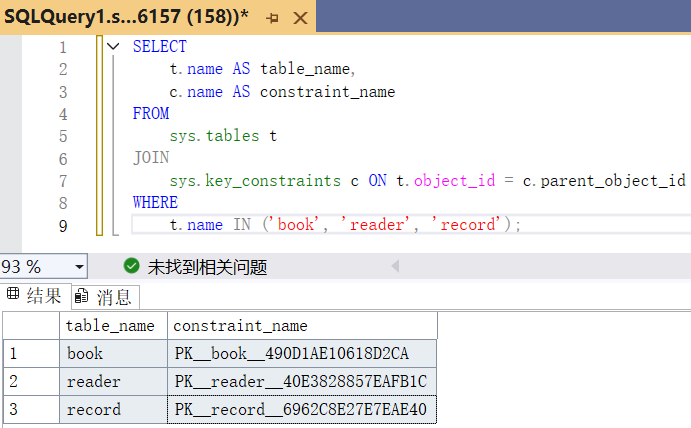
\includegraphics[width=0.8\textwidth]{img/primary_key_query.png}
\caption{主键约束查询结果}
\label{fig:primary_key_query}
\end{figure}

\paragraph{实验前外键约束查询}
在进行外键约束删除和添加实验前，先查询当前book、borrow\_statistics、reader、reader2、record等表的外键约束情况，具体SQL如下：
\begin{lstlisting}[language=SQL, caption=查询外键约束]
SELECT 
    fk.name AS ForeignKeyName,
    fk.parent_object_id AS ParentObjectId,
    OBJECT_NAME(fk.parent_object_id) AS ParentObjectName,
    fk.referenced_object_id AS ReferencedObjectId,
    OBJECT_NAME(fk.referenced_object_id) AS ReferencedObjectName,
    fkc.parent_column_id,
    col.name AS ParentColumnName,
    fkc.referenced_column_id,
    refcol.name AS ReferencedColumnName
FROM 
    sys.foreign_keys AS fk
INNER JOIN 
    sys.foreign_key_columns AS fkc ON fk.object_id = fkc.constraint_object_id
INNER JOIN 
    sys.columns AS col ON fkc.parent_column_id = col.column_id AND fkc.parent_object_id = col.object_id
INNER JOIN 
    sys.columns AS refcol ON fkc.referenced_column_id = refcol.column_id AND fkc.referenced_object_id = refcol.object_id
WHERE 
    OBJECT_NAME(fk.parent_object_id) IN ('book', 'borrow_statistics', 'reader', 'reader2', 'record');
\end{lstlisting}
\begin{figure}[H]
\centering
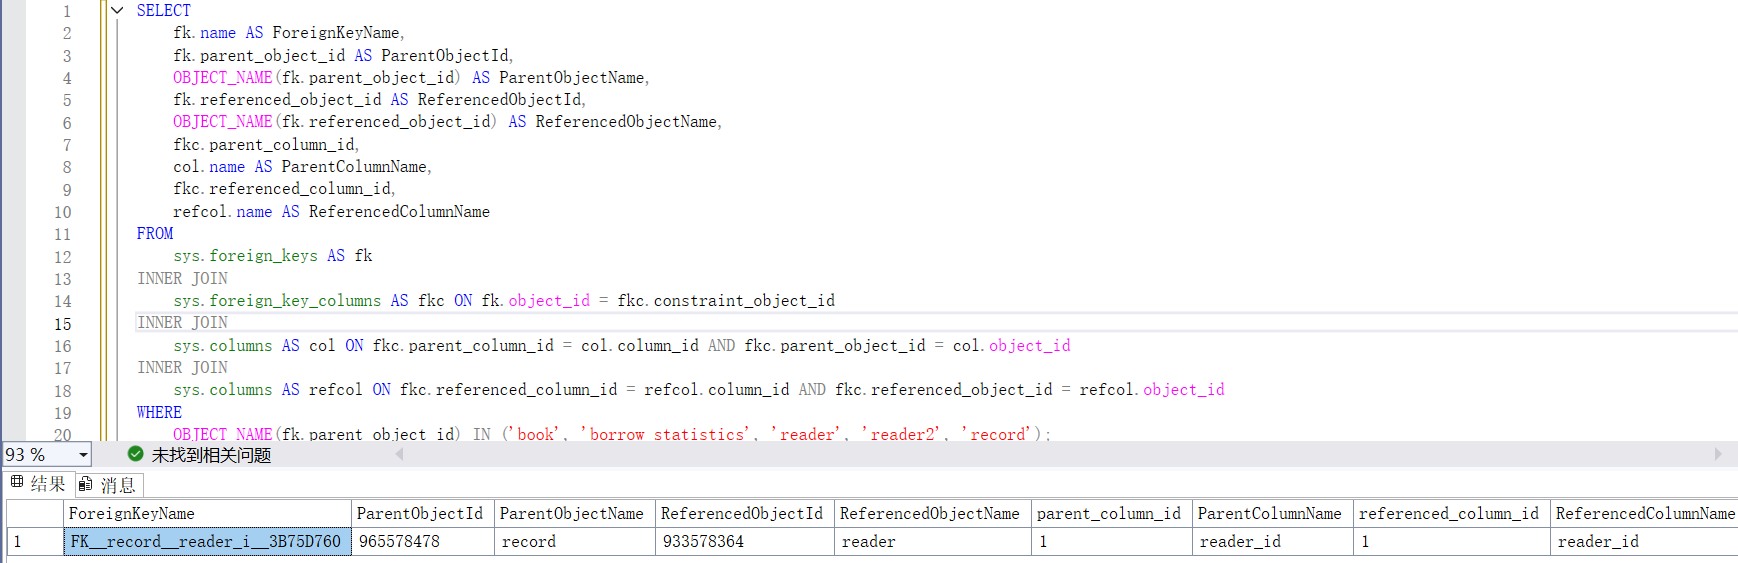
\includegraphics[width=0.8\textwidth]{img/foreign_key_query.png}
\caption{外键约束查询结果}
\label{fig:foreign_key_query}
\end{figure}

查询外键约束后，可以根据实际外键名进行删除。
\begin{lstlisting}[language=SQL, caption=删除指定外键约束]
ALTER TABLE dbo.record DROP CONSTRAINT FK__record__reader_i__3B75D760;
\end{lstlisting}

\paragraph{a) 删除主键约束}
使用ALTER TABLE语句分别对book表、reader表和record表删除主键约束。具体操作如下：
\begin{lstlisting}[language=SQL, caption=删除主键约束]
ALTER TABLE book DROP CONSTRAINT PK__book__490D1AE10618D2CA;
ALTER TABLE reader DROP CONSTRAINT PK__reader__40E3828857EAFB1C;
ALTER TABLE record DROP CONSTRAINT PK__record__6962C8E27E7EAE40;
\end{lstlisting}

删除后查询主键约束情况：
\begin{lstlisting}[language=SQL, caption=删除主键后查询主键约束]
SELECT 
    t.name AS table_name,
    c.name AS constraint_name
FROM 
    sys.tables t
JOIN 
    sys.key_constraints c ON t.object_id = c.parent_object_id
WHERE 
    t.name IN ('book', 'reader', 'record');
\end{lstlisting}
\begin{figure}[H]
\centering
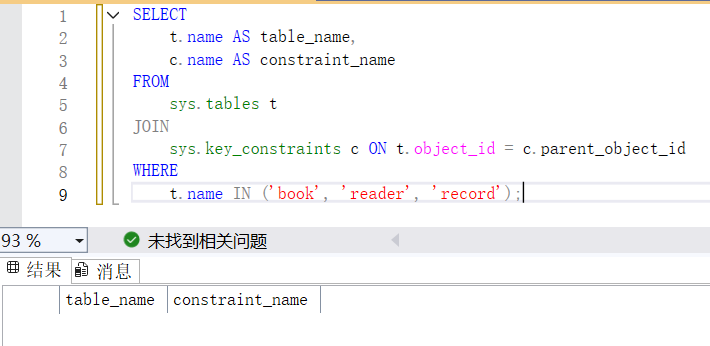
\includegraphics[width=0.8\textwidth]{img/primary_key_drop_result.png}
\caption{删除主键约束后的查询结果}
\label{fig:primary_key_drop_result}
\end{figure}

\paragraph{b) 添加主键约束}
使用ALTER TABLE语句分别对book表、reader表和record表添加主键约束。约束名分别为：book表的主键约束名为PRK\_Book，reader表约束名为PRK\_Reader，record表主键约束名为PRK\_Record。具体操作如下：
\begin{lstlisting}[language=SQL, caption=添加主键约束]
ALTER TABLE book ADD CONSTRAINT PRK_Book PRIMARY KEY (book_id);
ALTER TABLE reader ADD CONSTRAINT PRK_Reader PRIMARY KEY (reader_id);
ALTER TABLE record ADD CONSTRAINT PRK_Record PRIMARY KEY (borrow_date);
\end{lstlisting}

添加后查询主键约束情况：
\begin{lstlisting}[language=SQL, caption=添加主键后查询主键约束]
SELECT 
    t.name AS table_name,
    c.name AS constraint_name
FROM 
    sys.tables t
JOIN 
    sys.key_constraints c ON t.object_id = c.parent_object_id
WHERE 
    t.name IN ('book', 'reader', 'record');
\end{lstlisting}
\begin{figure}[H]
\centering
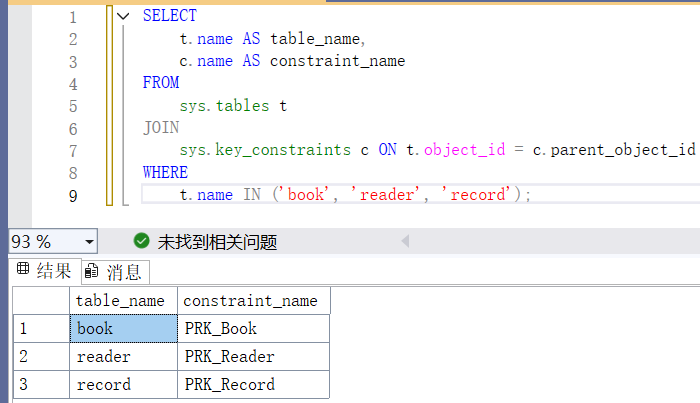
\includegraphics[width=0.8\textwidth]{img/primary_key_add_result.png}
\caption{添加主键约束后的查询结果}
\label{fig:primary_key_add_result}
\end{figure}

\paragraph{c) 插入记录验证主键约束}
在三个表中分别插入与已有主键重复的记录，验证主键约束是否生效，能够阻止重复主键的插入。具体操作如下：
\begin{lstlisting}[language=SQL, caption=插入重复主键记录验证约束]
INSERT INTO book VALUES ('b0001', '重复主键书', '978-7-000-00000-0', '张三', '测试出版社', 1, 10.00); -- 应失败
INSERT INTO reader VALUES ('r0001', '重复主键读者', '男', '测试地址'); -- 应失败
INSERT INTO dbo.record (reader_id, book_id, borrow_date, return_date, notes)
VALUES (CONVERT(VARCHAR, 'r0001'), CONVERT(VARCHAR, 'b0003'), CONVERT(DATE, '2014-01-12'), CONVERT(DATE, '2014-01-12'), NULL); -- 应失败
\end{lstlisting}

插入后查询表数据（以book为例）：
\begin{lstlisting}[language=SQL, caption=插入后查询book表数据]
SELECT * FROM book;
\end{lstlisting}
\begin{figure}[H]
\centering
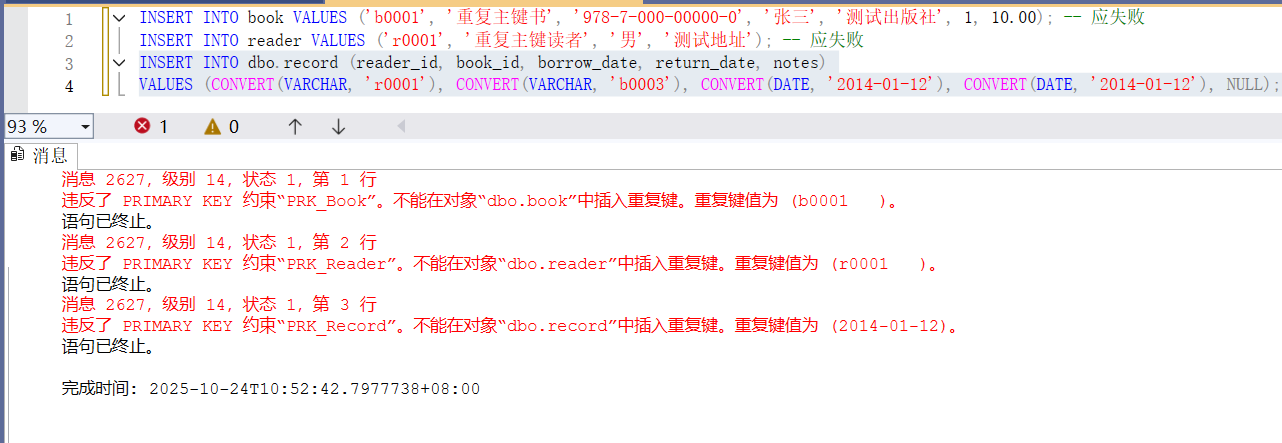
\includegraphics[width=0.8\textwidth]{img/primary_key_insert_result.png}
\caption{插入重复主键后的表数据查询结果}
\label{fig:primary_key_insert_result}
\end{figure}

\subsubsection{2. 添加与删除外键约束}

\paragraph{a) 删除外键约束}
使用ALTER TABLE语句对record表删除外键约束，分别删除book\_id和reader\_id上的外键约束。具体操作如下：
\begin{lstlisting}[language=SQL, caption=删除外键约束]
ALTER TABLE record DROP CONSTRAINT FK_record_book;
ALTER TABLE record DROP CONSTRAINT FK_record_reader;
ALTER TABLE dbo.record DROP CONSTRAINT FK__record__reader_i__3B75D760;
\end{lstlisting}

删除后查询外键约束情况：
\begin{lstlisting}[language=SQL, caption=删除外键后查询外键约束]
SELECT 
    fk.name AS ForeignKeyName,
    OBJECT_NAME(fk.parent_object_id) AS ParentObjectName
FROM 
    sys.foreign_keys AS fk
WHERE 
    OBJECT_NAME(fk.parent_object_id) IN ('record');
\end{lstlisting}
\begin{figure}[H]
\centering
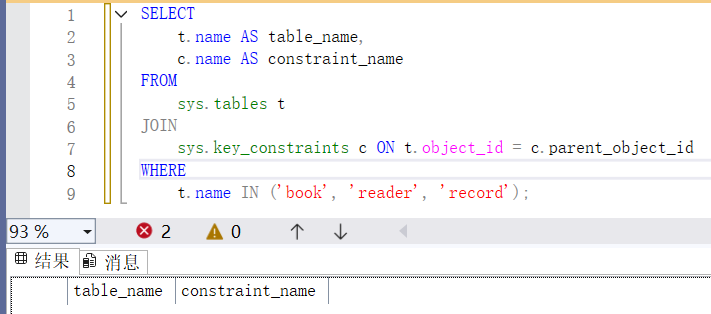
\includegraphics[width=0.8\textwidth]{img/foreign_key_drop_result.png}
\caption{删除外键约束后的查询结果}
\label{fig:foreign_key_drop_result}
\end{figure}

\paragraph{b) 添加外键约束（ON DELETE/UPDATE SET NULL）}
使用ALTER TABLE语句对record表添加外键约束，分别关联book表的book\_id和reader表的reader\_id。设置ON DELETE SET NULL和ON UPDATE SET NULL，即当被参照表的记录被删除或修改时，record表中对应字段值自动设为NULL。具体操作如下：
\begin{lstlisting}[language=SQL, caption=添加外键约束]
ALTER TABLE record
ADD CONSTRAINT FK_record_book FOREIGN KEY (book_id)
REFERENCES book(book_id)
ON DELETE SET NULL ON UPDATE SET NULL;

ALTER TABLE record
ADD CONSTRAINT FK_record_reader FOREIGN KEY (reader_id)
REFERENCES reader(reader_id)
ON DELETE SET NULL ON UPDATE SET NULL;
\end{lstlisting}

添加后查询外键约束情况：
\begin{lstlisting}[language=SQL, caption=添加外键后查询外键约束]
SELECT 
    fk.name AS ForeignKeyName,
    OBJECT_NAME(fk.parent_object_id) AS ParentObjectName
FROM 
    sys.foreign_keys AS fk
WHERE 
    OBJECT_NAME(fk.parent_object_id) IN ('record');
\end{lstlisting}
\begin{figure}[H]
\centering
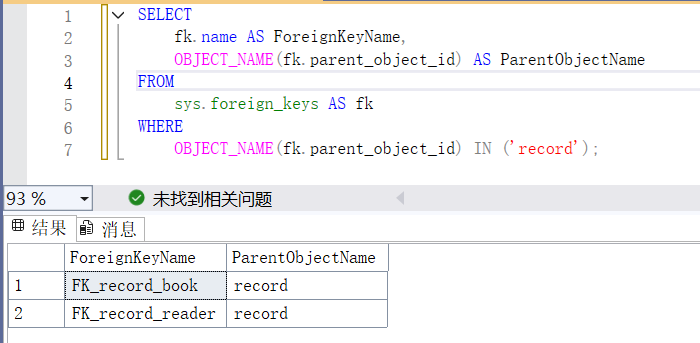
\includegraphics[width=0.8\textwidth]{img/foreign_key_add_result.png}
\caption{添加外键约束后的查询结果}
\label{fig:foreign_key_add_result}
\end{figure}

\subsubsection{3. 设置唯一性约束}

使用ALTER TABLE语句对book表的book\_name列添加唯一性约束，约束名为un\_name，保证book\_name值不重复。具体操作如下：
\begin{lstlisting}[language=SQL, caption=添加唯一性约束]
ALTER TABLE book ADD CONSTRAINT un_name UNIQUE (book_name);
\end{lstlisting}

添加后查询唯一性约束情况：
\begin{lstlisting}[language=SQL, caption=查询唯一性约束]
SELECT 
    i.name AS index_name, 
    OBJECT_NAME(i.object_id) AS table_name, 
    i.is_unique
FROM 
    sys.indexes i
WHERE 
    OBJECT_NAME(i.object_id) = 'book' AND i.is_unique = 1;
\end{lstlisting}
\begin{figure}[H]
\centering
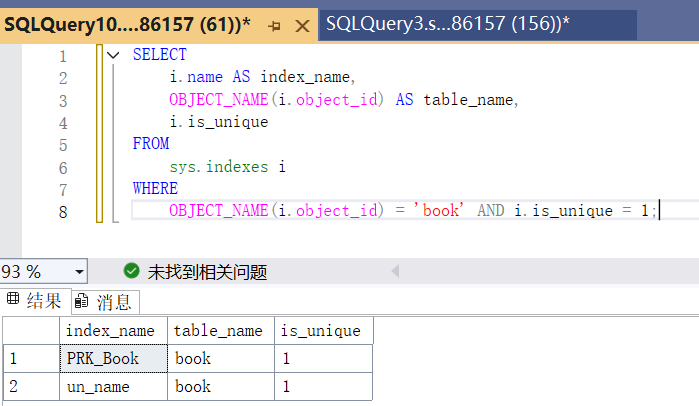
\includegraphics[width=0.8\textwidth]{img/unique_add_result.png}
\caption{添加唯一性约束后的查询结果}
\label{fig:unique_add_result}
\end{figure}

\subsubsection{4. 删除唯一性约束}

使用ALTER TABLE语句对book表删除book\_name上的唯一性约束un\_name。具体操作如下：
\begin{lstlisting}[language=SQL, caption=删除唯一性约束]
ALTER TABLE book DROP CONSTRAINT un_name;
\end{lstlisting}

删除后查询唯一性约束情况：
\begin{lstlisting}[language=SQL, caption=删除唯一性后查询唯一性约束]
SELECT 
    i.name AS index_name, 
    OBJECT_NAME(i.object_id) AS table_name, 
    i.is_unique
FROM 
    sys.indexes i
WHERE 
    OBJECT_NAME(i.object_id) = 'book' AND i.is_unique = 1;
\end{lstlisting}
\begin{figure}[H]
\centering
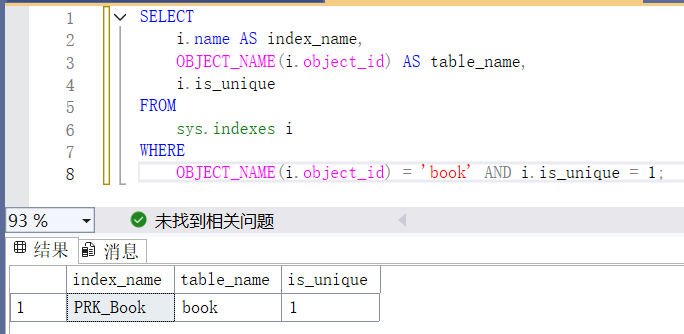
\includegraphics[width=0.8\textwidth]{img/unique_drop_result.png}
\caption{删除唯一性约束后的查询结果}
\label{fig:unique_drop_result}
\end{figure}

\subsubsection{5. 设置检查约束}

使用ALTER TABLE语句对book表的book\_id列添加检查约束，约束名为ck\_idb，要求book\_id必须符合'b[0-9][0-9][0-9][0-9]'格式。具体操作如下：
\begin{lstlisting}[language=SQL, caption=添加检查约束]
ALTER TABLE book ADD CONSTRAINT ck_idb CHECK (book_id LIKE 'b[0-9][0-9][0-9][0-9]');
\end{lstlisting}

添加后查询检查约束情况：
\begin{lstlisting}[language=SQL, caption=查询检查约束]
SELECT 
    OBJECT_NAME(parent_object_id) AS table_name, 
    name AS constraint_name, 
    type_desc
FROM 
    sys.check_constraints
WHERE 
    OBJECT_NAME(parent_object_id) = 'book';
\end{lstlisting}
\begin{figure}[H]
\centering
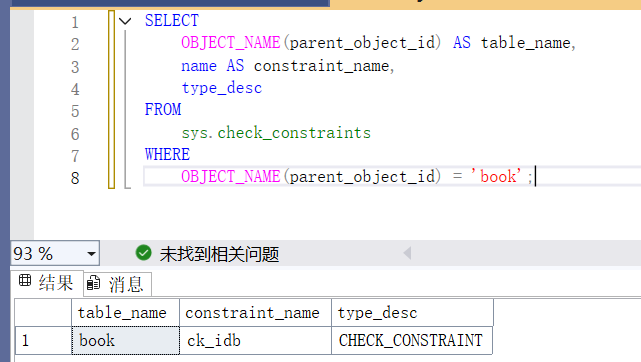
\includegraphics[width=0.8\textwidth]{img/check_add_result.png}
\caption{添加检查约束后的查询结果}
\label{fig:check_add_result}
\end{figure}

\subsubsection{6. 创建规则并绑定到reader表}

创建规则rule\_sex，规定插入或更新reader表reader\_sex字段的值只能为‘男’或‘女’，并将该规则绑定到reader表的reader\_sex字段。具体操作如下：
\begin{lstlisting}[language=SQL, caption=创建规则并绑定]
CREATE RULE rule_sex AS @value IN ('男', '女');
GO

-- 将规则绑定到reader表的reader_sex字段
EXEC sp_bindrule 'rule_sex', 'reader.reader_sex';
GO
\end{lstlisting}

创建并绑定后查询规则绑定情况：
\begin{lstlisting}[language=SQL, caption=查询规则绑定]
SELECT name, definition 
FROM sys.sql_modules m
JOIN sys.objects o ON m.object_id = o.object_id
WHERE o.type = 'R' AND o.name = 'rule_sex';
\end{lstlisting}
\begin{figure}[H]
\centering
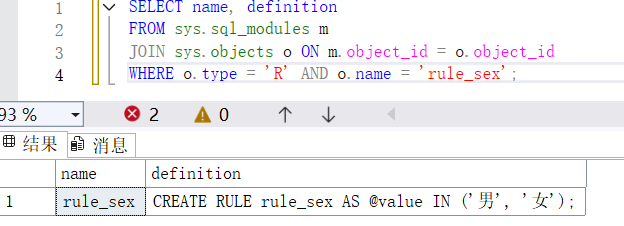
\includegraphics[width=0.8\textwidth]{img/rule_bind_result.png}
\caption{规则绑定后的查询结果}
\label{fig:rule_bind_result}
\end{figure}

\subsubsection{7. 验证CHECK约束和规则}

插入或修改记录，分别验证book表的book\_id检查约束和reader表的reader\_sex规则是否生效。具体操作如下：
\begin{lstlisting}[language=SQL, caption=插入/修改记录验证约束]
INSERT INTO book VALUES ('b1234', '新书', '978-7-000-00001-1', '李四', '出版社', 1, 20.00); -- 应成功
INSERT INTO book VALUES ('x1234', '非法ID书', '978-7-000-00002-2', '王五', '出版社', 1, 20.00); -- 应失败

INSERT INTO reader VALUES ('r1234', '测试读者', '男', '地址'); -- 应成功
INSERT INTO reader VALUES ('r1235', '测试读者2', '未知', '地址'); -- 应失败
UPDATE reader SET reader_sex = '女' WHERE reader_id = 'r1234'; -- 应成功
UPDATE reader SET reader_sex = 'abc' WHERE reader_id = 'r1234'; -- 应失败
\end{lstlisting}

结果截图留空
\begin{figure}[H]
\centering
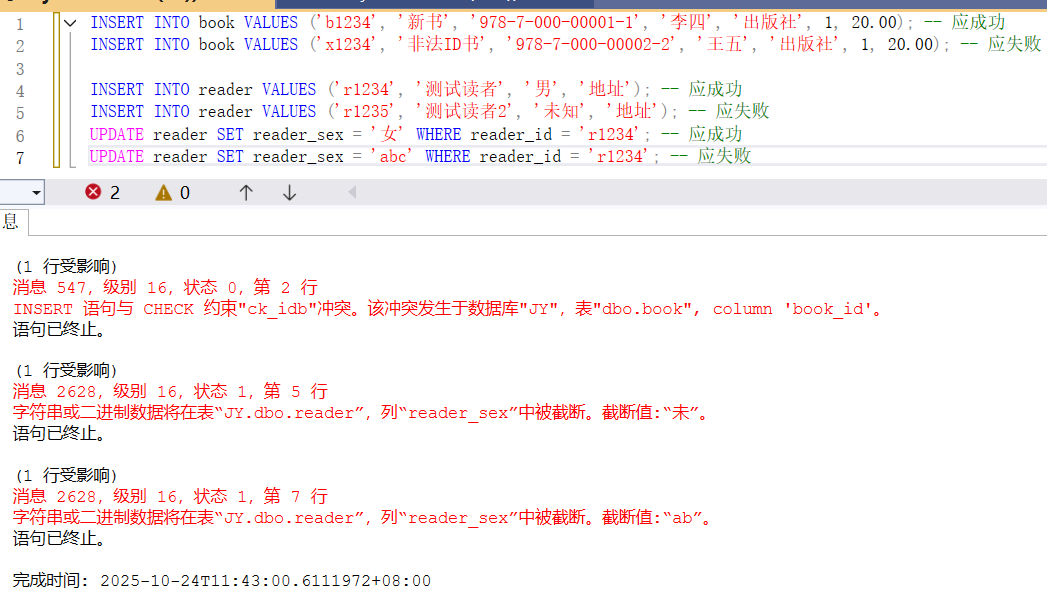
\includegraphics[width=0.8\textwidth]{img/check_rule_test.png}
\caption{CHECK约束与规则验证结果}
\label{fig:check_rule_test}
\end{figure}

\subsection{总结与思考}
\subsubsection{总结}
通过本次实验，掌握了数据库完整性约束的相关操作，包括主键、外键、唯一性、检查约束和规则的创建与删除。实体完整性、参照完整性和用户自定义约束的设置，有效保证了数据库数据的正确性和一致性。实验过程中，验证了各类约束的实际效果，加深了对数据库完整性机制的理解。

\subsubsection{困难和解决}

在实验过程中遇到了几个技术难点，通过分析错误信息和查阅文档，最终找到了解决方案：

\paragraph{1. 数据类型不匹配问题}
在创建外键约束时遇到错误：
\begin{quote}
消息 1778，级别 16，状态 0，第 1 行
列 'book.book\_id' 的数据类型与外键 'FK\_record\_book' 中的引用列 'record.book\_id' 的数据类型不同。
\end{quote}

\textbf{问题分析：}通过查询发现数据类型不匹配：
\begin{itemize}
\item book.book\_id: CHAR(8)
\item record.book\_id: VARCHAR(10) 
\item reader.reader\_id: CHAR(8)
\item record.reader\_id: VARCHAR(10)
\end{itemize}

\textbf{解决方案：}修改record表的列数据类型以匹配主表：
\begin{lstlisting}[language=SQL, caption=修改数据类型解决外键约束问题]
-- 删除现有的外键约束
IF EXISTS (SELECT * FROM sys.foreign_keys WHERE name = 'FK_record_book')
    ALTER TABLE record DROP CONSTRAINT FK_record_book;

-- 修改record表的列数据类型以匹配主表
ALTER TABLE record ALTER COLUMN book_id CHAR(8) NULL;
ALTER TABLE record ALTER COLUMN reader_id CHAR(8) NULL;

-- 重新添加外键约束
ALTER TABLE record
ADD CONSTRAINT FK_record_book FOREIGN KEY (book_id)
REFERENCES book(book_id)
ON DELETE SET NULL ON UPDATE SET NULL;
\end{lstlisting}

\paragraph{2. 日期格式转换问题}
在插入日期数据时遇到格式解析错误。

\textbf{解决方案：}使用CONVERT函数确保日期格式正确：
\begin{lstlisting}[language=SQL, caption=使用CONVERT函数处理日期格式]
INSERT INTO dbo.record (reader_id, book_id, borrow_date, return_date, notes)
VALUES (CONVERT(VARCHAR, 'r0001'), CONVERT(VARCHAR, 'b0003'), 
        CONVERT(DATE, '2014-01-12'), CONVERT(DATE, '2014-01-12'), NULL);
\end{lstlisting}

\paragraph{3. SET NULL引用操作约束问题}
在创建外键约束时遇到错误：
\begin{quote}
消息 1761，级别 16，状态 0，第 1 行
由于一个或多个引用列不可为 Null，因此无法使用 SET NULL 引用操作创建外键
\end{quote}

\textbf{问题分析：}主键列默认不允许NULL值，但SET NULL操作要求被引用列可以为NULL。

\textbf{解决方案：}
\begin{lstlisting}[language=SQL, caption=处理SET NULL约束问题]
-- 1. 删除主键约束
ALTER TABLE dbo.book DROP CONSTRAINT PRK_Book;

-- 2. 修改列允许NULL值（如果业务逻辑允许）
ALTER TABLE dbo.book ALTER COLUMN book_id CHAR(8) NULL;

-- 3. 重新添加主键约束（如果需要保持主键特性）
ALTER TABLE dbo.book ADD CONSTRAINT PRK_Book PRIMARY KEY (book_id);
\end{lstlisting}

这些问题的解决过程让我深入理解了SQL Server中数据类型匹配、约束冲突处理和外键引用操作的具体机制，为今后的数据库设计和维护积累了宝贵经验。

\end{document}